\documentclass{bcthesis}

%%% Other packages needed by your document may be loaded here.
\usepackage{url}              % For formatting URLs 
\usepackage{booktabs}         % Publication-quality tables.
\usepackage[square]{natbib}           % Provides some nice citation and
							  % bibliography formatting commands.
% \bibpunct[:~]{(}{)}{;}{a}{,}{,~} % Set some defaults for bibliographic
								 % punctuation used by natbib.sty.
\usepackage{verbatim}
\usepackage{graphicx}
\usepackage{subfig} % Because subcaption does not seem to be compatible with the template.
\usepackage{calc}
\usepackage{textcomp}
\usepackage{amsfonts}
\usepackage{amssymb}
\usepackage{tikz}
\usepackage{float}
% \usepackage{showframe}
\usepackage{james}
\usepackage[plainpages=false,pdfpagelabels, hidelinks]{hyperref}

\usetikzlibrary{arrows, automata, shapes}

%%% Document Settings
	% The following command allows tables to split between pages:
	% \allowdisplaybreaks

	% Provide additional context around errors. 
	\setcounter{errorcontextlines}{1000}

	\setlength{\parskip}{0.5 em}

	\newif\ifbuildfrontmatter
	\buildfrontmatterfalse
	% \buildfrontmattertrue

	% Use this to toggle professionalism
	\newif\ifpresstime
	\presstimefalse
	\presstimetrue

	\ifpresstime
		\buildfrontmattertrue
		\renewcommand{\meo}[1]{}
		\allhrfalse
	\fi

	\tikzset{
		initial text = {\scriptsize{\textsc{start}}},
		initial distance = 1 pt,
		every initial by arrow/.style={->},
		elliptic state/.style={draw,rounded rectangle}
	}


%%% End document settings

%%% Begin information section 
	%% title of your report?
	\title{An Exemplified Proof of Kleene's Theorem}

	%% Your name 
	\author{James McFeeters}

	% Photo -- see bcthesis class line 168

	\advisor{Darrah Chavey}

	%% Second reader's name? Ask the Colloquium Instructor who it will be.
	\reader{Name of Second Reader}

	\thesisyear{2018}
	\thesismonth{April}
%%% End of information section.


%%% New Environments

%%% End new environments 

%%% New commands
	\newcommand{\footcite}[2]{\footnote{\cite[pg.~{#2}]{#1}}}
	\renewcommand{\footcite}[2]{\cite[pg.~{#2}]{#1}}
%%% End new commands


%%% The start of the document!
\begin{document}

\ifbuildfrontmatter
\frontmatter

	\maketitle

	\begin{abstract}
		\meo{This is a placeholder abstract!}

		This paper gives a standard proof of Kleene's theorem, with examples to help illuminate particular facets of the proof.
		Kleene's theorem establishes the equivalence of finite automata and the class of regular languages, allowing for the implementation of fast search algorithms using regular expressions.

		\meo{This is a placeholder abstract!}
	\end{abstract}


	%%% If you want to thank someone for their influence on your life or your work, here's where you'd do it.
	\begin{acknowledgments}
		Here you should acknowledge any special help on your project, or particular influences on your life or mathematical development.
	\end{acknowledgments}

	%%% Table of Contents, List of Figures, and List of Tables. 
	% If you don't have any figures or tables in your report, you can
	% comment out the appropriate command.
	\tableofcontents
	% \listoffigures
	% \listoftables
%%% End of the front matter.
\fi

%%% Beginnning of the main matter.
\mainmatter

\mychapter{Basic Definitions}
\label{ch:basics}

		\begin{definition}[Symbol]
			The \textit{symbol} is the most basic unit of formal language theory.
			Symbols are indivisible and atomic --- they are not a composite of other units, and cannot be represented by any combination of other symbols.\footcite{hopcroft}{1}
		\end{definition}

		\begin{definition}[Alphabet]
			An \textit{alphabet} is a nonempty and finite set of symbols.
			An alphabet is typically denoted by the symbol $\Sigma$.\footcite{salomaa}{1}
		\end{definition}

		\begin{definition}[String]
			A \textit{string} over an alphabet $\Sigma$ is a finite sequence of symbols of $\Sigma$.
			If $\Sigma = \{ a, b ,c \}$, then $w = abbc$ is a string over $\Sigma$.
			The length of a string is the number of symbols it contains, counting repetitions.
			The length of $w$, denoted $|w|$, is $4$.
			Strings are also referred to as \textit{words}.\footcite{hopcroft}{1}

			The string of length zero, which contains no symbols, is called the \textit{empty string}, and denoted $\lambda$.
			The empty string is a valid string over any alphabet.\footcite{salomaa}{1}
		\end{definition}

		\begin{definition}[Language]
			A \textit{language} over an alphabet $\Sigma$ is any set of strings over $\Sigma$.\footcite{hopcroft}{2}
			% The language of all possible strings over $\Sigma$ is denoted $\Sigma^*$.

			The empty set ($\emptyset$) and $\{ \lambda \}$ are valid languages over any alphabet.\footcite{hopcroft}{2}

			Because languages are sets of strings, the conventional set operations, such as union, intersection, and complementation are defined for languages.\footcite{hopcroft}{5}
		\end{definition}

		\begin{remark}
			The empty set and $\{ \lambda \}$ represent distinct languages. 
			The empty set represents the language containing no strings at all, while $\{ \lambda \}$ represents the language containing only the empty string.\footcite{hopcroft}{2}
		\end{remark}


\mychapter{Regular Expressions} % (fold)
\label{ch:regular_expressions}
	
	\begin{definition}[Atomic Regular Languages]
		The \textit{atomic regular languages} are the basic units used to build all other regular languages.
		They are defined for any alphabet $\Sigma$ as follows:
		\begin{enumerate}[label=(\roman*), itemsep = -0.3 ex]
			\item $\emptyset$ is an atomic regular language over $\Sigma$.
			\item $\{ \lambda \}$ is an atomic regular language over $\Sigma$.
			\item $\{ a \}$ is an atomic regular language over $\Sigma$ for all $a \in \Sigma$.
		\end{enumerate}
		\footcite{hopcroft}{28}
	\end{definition}

	We now define the operations used to combine the atomic regular languages to form more complex regular languages.

	\begin{definition}[Concatenation]
		Let $w_1 = ab$ and $w_2 = bc$ be strings over some alphabet.
		Their \textit{concatenation} $w_1 w_2$ denotes the string $abbc$, and $w_2 w_1$ denotes $bcab$.
		For any string $w$, $\lambda w = w \lambda = w$.
		The notation $w^3$ denotes the string $www$, and $w^0 = \lambda$.\footcite{salomaa}{1}

		It should be easy to see how this definition applies to symbols, which can be seen as words of length 1.
	\end{definition}

	\begin{definition}[Concatenation of Languages]
		Let $A$ and $B$ be languages over some alphabet.
		The\textit{concatenation}, or \textit{product}, $AB$ of $A$ and $B$ is the set $\{ ab \mid a \in A, \ b \in B \}$.\footcite{lemmings}{3}

		The notation $A^2$ represents the language $AA$, and $A_i$ represents $AA^{i-1}$
		Note that $A = A^1 = AA^0 = \{ a \lambda \mid a \in A \}$, which implies that $A^0 = \{ \lambda \}$.\footcite{lemmings}{3}
	\end{definition}

	\begin{remark}
		Note that the set of strings over an alphabet is closed under concatenation: if $x$ and $y$ are strings over $\Sigma$, then so are $xy$ and $yx$.
		It follows that if $A$ and $B$ are languages over $\Sigma$, then so are $AB$ and $BA$.\footcite{lemmings}{2}
		
		Concatenation is also an associative operation.
		Given strings $x$, $y$, and $z$, $(xy)z = x(yz)$.
		It follows that for languages $A$, $B$, and $C$, $(AB)C = A(BC)$.\footcite{lemmings}{2}

		\meo{
			Maybe also note that length has the properties of the logarithm with regard to concatenation.
			It's a curiosity, but not really useful information
		}
	\end{remark}

	\begin{definition}[Kleene Closure]
		Given any language $A$, the language 
		\[
			A^* = \bigcup_{i \geq 0} A^i
		\]
		is called the \textit{Kleene closure} of $A$.
		$A^*$ is the language any words of $A$ repeated zero or more times, thus $\lambda$ is in the Kleene closure of any language.\footcite{lemmings}{3}
		\meo{Maybe note that that the star operator is referred to as the Kleene star.}
	\end{definition}

	\begin{definition}[Regular Language]
		Given an alphabet $\Sigma$, any atomic regular language over $\Sigma$ is a regular language over $\Sigma$.
		
		If $A$ and $B$ are regular languages over $\Sigma$, then so are 
		\begin{enumerate}[label=(\roman*), itemsep = -0.3 ex, nolistsep]
			\item $AB$
			\item $A \cup B$
			\item $A^*$
		\end{enumerate}
		\footcite{rosen}{879}
	\end{definition}

	\begin{remark}
		Because of their relationship to the family of regular languages, the concatenation, union, and Kleene closure are referred to as the \textit{regular operations}.\footcite{salomaa}{26}
	\end{remark}

	We now introduce \textit{regular expressions}, a shorthand used to describe regular languages.

	\begin{definition}[Regular Expressions]
		The atomic regular expressions over an alphabet $\Sigma$ are defined to represent the atomic regular languages over $\Sigma$:
		\begin{enumerate}[label=(\roman*), itemsep = -0.3 ex, nolistsep]
			\item $\emptyset$ denotes the empty language
			\item $\lambda$ denotes the language $\{ \lambda \}$
			\item $a$ denotes the language $\{ a \}$ for all $a \in \Sigma$
		\end{enumerate}
		\footcite{hopcroft}{28--29}

		If $\alpha$ and $\beta$ are regular expressions representing languages $A$ and $B$, respectively, then the following are also regular expressions:
		\begin{enumerate}[label=(\roman*), itemsep = -0.3 ex, nolistsep]
			\item $\alpha \beta$ denotes the language $AB$.
			\item $\alpha + \beta$ denotes the language $A \cup B$.
			\item $\alpha^*$ denotes the language $A^*$.
		\end{enumerate}
		\footcite{hopcroft}{28--29}
	\end{definition}

	\begin{remark}
		Although regular expressions may closely resemble the the notation for regular languages, they are in fact only a shorthand used to describe regular language. 
		Using regular expressions allows us to describe regular languages while avoiding some of the formalisms of set notation.
		\meo{
			Is this a convincing reason why this is a thing worth having?
			Maybe mention that a language is regular if and only if it can be described by a regular expression.
		}

	\end{remark}

	\meo{
		I could mention here that regular expressions are an example of a grammar, shockingly belonging to the class of regular grammars.
	}

% chapter regular_expressions (end)

\mychapter{Finite Automata} % (fold)
\label{ch:finite_automata}

	A finite automaton is a formal model of a machine which has a finite number of allowed configurations, called states, and accepts input symbols from some finite alphabet. 
	Each time a symbol is input to the automaton, it may transition to a new state. 
	The output of a finite automaton is the state of the machine after reading some input.

	\begin{definition}[Finite Automaton]
		A \textit{finite automaton} (FA) $M$ is defined by the 5-tuple $(Q, \Sigma, s, \delta, F)$.
		\begin{itemize}
			\item [] $Q$ is a finite and nonempty set of states.
			\item [] $\Sigma$ is an alphabet of possible input symbols.
			\item [] $s \in Q$ is the state of the machine prior to any input, referred to as the \textit{initial state};
			\item [] $\delta: (Q \times \Sigma) \mapsto Q$ is called the \textit{transition function}: It maps a starting state and an input symbol to the new state of the machine.
			\item [] $F \subseteq Q$ is the set of \textit{final states} or \textit{accepting states} of the machine.
		\end{itemize}
		\footcite{hopcroft}{17}
	\end{definition}

	\begin{remark}
		It is convenient to extend the definition of $\delta$ to apply to strings, as well as individual symbols.
		Let $w = w_1 w_2 \dots w_n$.
		By 
		\[
			\delta(q_1, w) = q_n
		\] 
		we mean 
		\[
			\delta\bigg( \cdots \ \delta\Big( \ \delta(q_1, w_1), \ w_2 \Big), \cdots, w_n \bigg) = q_n.
		\]
		We define $\delta(q_i, \lambda) = q_i$.
		This defines $\delta: (Q \times \Sigma^*) \mapsto Q$.\footcite{hopcroft}{17}
	\end{remark}

	\begin{definition}(Acceptance by Finite Automaton)
		Let $M = (Q, \Sigma, q_0, \delta, F)$ be an FA and let $w \in \Sigma^*$.
		We say that $w$ is \textit{accepted} by $M$ if $\delta(q_0, w) \in F$.\footcite{hopcroft}{18}

		We use $L(M)$ to denote the language $\{ w \in \Sigma^* \mid \delta(q_0, w) \in F \}$ containing all strings accepted by $M$.\footcite{hopcroft}{18}

		A language $A$ is considered \textit{representable} if there exists some FA $M_A$ such that $A = L(M_A)$.\footcite{salomaa}{20}
	\end{definition}

	\begin{example}[Finite Automata Construction]

		% I'm ducking done typing ``shift-m, shift-underscore, 3''. 
		\newcommand{\miii}{\ensuremath{M_3}\xspace}

		To illustrate exactly how the components of an FA function, we will give a step-by-step construction of an FA to recognize the language of binary numbers divisible by 3.

		Call this automaton \miii.
		Let $\miii = (Q, \Sigma, s, \delta, F)$.
		Clearly we need only the symbols ``0'' and ``1'' to represent a language of binary strings, so we set $\Sigma = \{ 0, 1 \}$.

		Now we define the set of states for $\miii$.
		Suppose $x$ is the string that has been input to $\miii$ so far.
		It is clear that for any $x$, exactly one of the following must be true:
		\begin{itemize}[itemsep = -1 ex, nolistsep]
			\item [] $x = 0 \mod 3$,
			\item [] $x = 1 \mod 3$,
			\item [] $x = 2 \mod 3$.
		\end{itemize}
		So we create one state to represent each of these possible conditions, and define $Q = \{ q_0, q_1, q_2 \}$.
		Since we want $\miii$ to accept numbers divisible by 3, we set $F = \{ q_0 \}$. 
		And since we interpret no input as 0, set the initial state $s$ to $q_0$.

		Now we have 
		\[
			\miii = (Q = \{ q_0, q_1, q_2 \}, \Sigma = \{ 0, 1 \}, s = q_0, \delta, F = \{ q_0 \}).
		\]
		The only part of \miii remaining to be defined is $\delta$, the transition function.

		To define the transition function $\delta$ it is helpful to have a picture of the automaton we are building.
		We draw FAs as directed graphs, with vertices representing states and edges, labeled by symbols, representing transitions.
		A double circle around a vertex means that it represents an accepting state.

		Figure~\ref{fig:m3_1} shows $\miii$ as defined thus far: lacking any transitions, but otherwise complete.


		\begin{figure}[H]
			\centering
			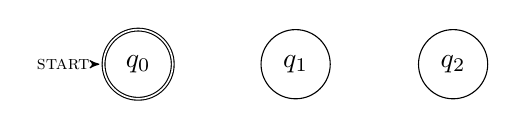
\begin{tikzpicture}[>=stealth',shorten >=1pt,auto,node distance=2cm]
				\node[initial,state,accepting] (0)                {$q_0$};
				\node[state]                   (1) [right of = 0] {$q_1$};
				\node[state]                   (2) [right of = 1] {$q_2$};
			\end{tikzpicture}
			\caption{$\miii$ without any transitions}
			\label{fig:m3_1}
		\end{figure}

		To define transitions, we imagine starting with the FA in its initial state and entering a string one symbol at a time.
		Each time we enter a symbol we decide what the next state of the machine should be, given the input so far, and then define a transition to produce that state.

		Suppose that $\miii$ is in its initial state.
		If the first input symbol is ``0'', then the machine should not change state.
		So we define $\delta(q_0, 0) = q_0$.
		If the first symbol is ``1'', the value of the input is $1$, so the next state should be $q_1$, and we define $\delta(q_0, 1) = q_1$.
		Figure~\ref{fig:m3_2} shows the automaton with these transitions added.

		\begin{figure}[H]
			\centering
			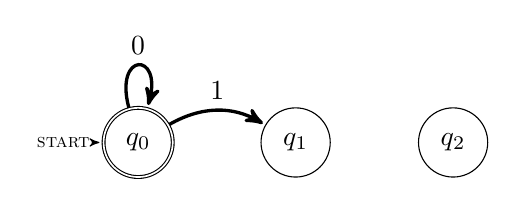
\begin{tikzpicture}[>=stealth',shorten >=1pt,auto,node distance=2cm]
				\node[initial,state,accepting] (q0)                 {$q_0$};
				\node[state]                   (q1) [right of = q0] {$q_1$};
				\node[state]                   (q2) [right of = q1] {$q_2$};

				\path[->, very thick](q0) edge [loop above] node {0} (q0);
				\path[->, very thick](q0) edge [bend left]  node {1} (q1);
			\end{tikzpicture}
			\caption{$\miii$ with transitions from $q_0$ added.}
			\label{fig:m3_2}
		\end{figure}

		Clearly, we do not need to add any more transitions from $q_0$, so we move on to $q_1$.
		Imagine that the input so far is ``1'', so that $\miii$ will be in state $q_1$.
		If the next symbol is ``0'', we have $10_b = 2$, and the next state should be $q_2$.
		So we define $\delta(q_1, 0) = q_2$.
		But if the next symbol is ``1'', we have $11_b = 3$. 
		Then the next state should be $q_0$, so we define $\delta(q_1, 1) = q_0$.
		Figure~\ref{fig:m3_3} shows \miii with these transitions added. 


		\begin{figure}[H]
			\centering
			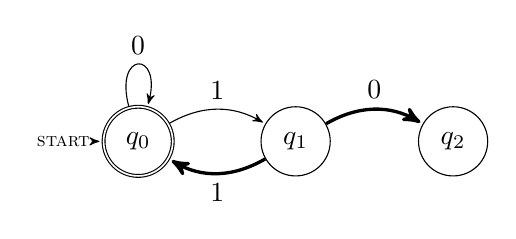
\begin{tikzpicture}[>=stealth',shorten >=1pt,auto,node distance=2cm]
				\node[initial,state,accepting] (q0)                {$q_0$};
				\node[state]                   (q1) [right of = q0] {$q_1$};
				\node[state]                   (q2) [right of = q1] {$q_2$};

				\path[->](q0) edge [loop above] node {0} (q0);
				\path[->](q0) edge [bend left]  node {1} (q1);
				\path[->, very thick](q1) edge [bend left]  node {0} (q2);
				\path[->, very thick](q1) edge [bend left]  node {1} (q0);
			\end{tikzpicture}
			\caption{\miii with transitions from $q_1$ added.}
			\label{fig:m3_3}
		\end{figure}

		Now we can define the transitions from $q_2$. 
		Imagine that the input so far is ``10''.
		If the next symbol is ``0'', we have $100_b = 4 \equiv 1 \mod 3$, so we define $\delta(q_2, 0) = q_1$.
		But if the next symbol is ``1'', we have $101_b = 5 \equiv 2 \mod 3$, so we set $\delta(q_2, 1) = q_2$.

		This completes the construction of \miii.
		Figure~\ref{fig:m3_4} shows the finished automaton.

		\begin{figure}[H]
			\centering
			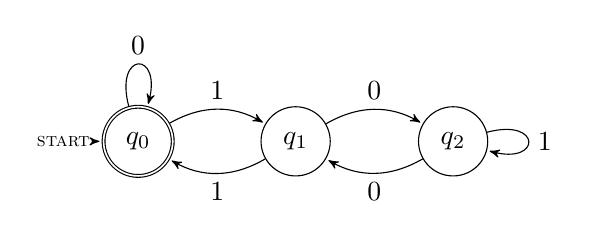
\begin{tikzpicture}[>=stealth',shorten >=1pt,auto,node distance=2cm]
				\node[initial,state,accepting] (q0)                {$q_0$};
				\node[state]                   (q1) [right of = q0] {$q_1$};
				\node[state]                   (q2) [right of = q1] {$q_2$};

				\path[->](q0) edge [loop above] node {0} (q0);
				\path[->](q0) edge [bend left]  node {1} (q1);
				\path[->](q1) edge [bend left]  node {0} (q2);
				\path[->](q1) edge [bend left]  node {1} (q0);
				\path[->](q2) edge [bend left]  node {0} (q1);
				\path[->](q2) edge [loop right] node {1} (q2);
			\end{tikzpicture}
			\caption{\miii with all its transitions.}
			\label{fig:m3_4}
		\end{figure}
	\end{example}

	\begin{definition}[Deterministic and Nondeterministic Finite Automata]
		Finite automata are divided into two classes: nondeterministic and deterministic finite automata.
		\begin{enumerate}[label=(\roman*)]
			\item A \textit{nondeterministic} finite automaton (NDFA) is an FA with \textit{zero or more} transitions from each state corresponding to each symbol in $\Sigma$.
			\item A \textit{deterministic} finite automaton (DFA) is an FA having \textit{exactly one} transition from each state corresponding to each symbol in $\Sigma$.
		\end{enumerate}
	\end{definition}

	\begin{remark}
		Because a DFA is required to have exactly one transition from each state for each possible input, only one of its states may be active at any given time.
		This is not the case for NDFAs.
		Because an NDFA may have any number of transitions from each state on a single symbol, any subset of its states may be active at any given time.
		Alternatively, an NDFA may have no transition from any state for a given input symbol, and upon reading that symbol would have no active states.

		an NDFA is considered to be in an accepting state when any of its accepting states are active.
		\meo{I could mention lambda transitions, but I've avoided using them so far, so I don't think I need to.}
	\end{remark}
% chapter finite_automata (end)


\mychapter{Kleene's Theorem} % (fold)
\label{ch:kleenes_theorem}

	\begin{theorem}[Kleene's Theorem]
		A language is representable if and only if it is regular.
	\end{theorem}

	\begin{claim}
	\label{prop:regular_languages_representable}
		All regular languages are representable.
	\end{claim}
	\begin{proof}
		We first show that the atomic regular languages are representable., then show that the results of the result of a regular operation on representable languages is representable.

		It is simple to construct an NDFAs to accept the atomic regular languages:
		\begin{itemize}
			\item [] $\emptyset$ is accepted by an automaton with one initial state, no accepting states, and no transitions, as depicted in Figure~\ref{sfig:ndfa_emptyset}.
			\item [] $\{ \lambda \}$ is accepted by the NDFA with one state, which is both its initial state and an accepting state, as in Figure~\ref{sfig:ndfa_lambda}.
			\item [] $\{ a \}$ for all $a \in \Sigma$ is accepted by an NDFA having two states: one initial state and one accepting state, with a transition on $a$ between them, as shown in Figure~\ref{sfig:ndfa_symbol}.
		\end{itemize}


		\begin{figure}[H]
			\centering
			\setlength{\fboxrule}{0 pt}
			\subfloat[NDFA accepting $\emptyset$]{
				\label{sfig:ndfa_emptyset}
				\framebox[0.3 \textwidth]{
					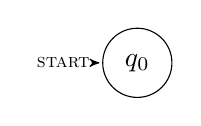
\begin{tikzpicture}[>=stealth',shorten >=1pt,auto,node distance=2cm]
						\node[initial,state] (q0)                {$q_0$};
					\end{tikzpicture}
				}
			}
			\subfloat[NDFA accepting $\{ \lambda \}$]{
				\label{sfig:ndfa_lambda}
				\framebox[0.3 \textwidth]{
					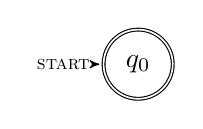
\begin{tikzpicture}[>=stealth',shorten >=1pt,auto,node distance=2cm]
						\node[initial,state, accepting] (q0)                {$q_0$};
					\end{tikzpicture}
				}
			}
			\subfloat[NDFA accepting $\{ a \}$ for all $a \in \Sigma$]{
				\label{sfig:ndfa_symbol}
				\framebox[0.3 \textwidth]{
					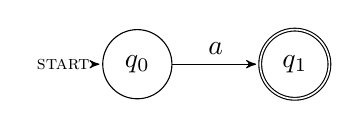
\begin{tikzpicture}[>=stealth',shorten >=1pt,auto,node distance=2cm]
						\node[initial,state]    (q0)                 {$q_0$};
						\node[state, accepting] (q1) [right of = q0] {$q_1$};
						\path[->](q0) edge  node {$a$} (q1);
					\end{tikzpicture}
				}
			}
			\caption{NDFAs representing the atomic regular languages}
			\label{fig:ndfa_atomic_regular_languages}
			% The \framebox makes the caption wider than the picture, 
			% otherwise, subfigures (a) and (b) are too narrow and their captions look bad.
		\end{figure}

		Now we must show that if $A$ and $B$ are representable languages, then so are
		\begin{enumerate}[label=(\roman*), itemsep = -0.3 ex, nolistsep]
			\item $AB$
			\item $A \cup B$
			\item $A^*$
		\end{enumerate}
		Starting with automata representing $A$ and $B$, we will construct automata to accept the regular operations applied to $A$ and $B$.

		% Commands to save me typing underscores everywhere
		% I want these scoped to the proof.
			\newcommand{\ma}{\ensuremath{M_A}\xspace}
				\newcommand{\qa}{\ensuremath{Q_A}\xspace}
				\newcommand{\siga}{\ensuremath{\Sigma_A}\xspace}
				\newcommand{\sa}{\ensuremath{s_A}\xspace}
				\newcommand{\dala}{\ensuremath{\delta_A}\xspace}
				\newcommand{\fa}{\ensuremath{F_A}\xspace}

			\newcommand{\mb}{\ensuremath{M_B}\xspace}
				\newcommand{\qb}{\ensuremath{Q_B}\xspace}
				\newcommand{\sigb}{\ensuremath{\Sigma_B}\xspace}
				\renewcommand{\sb}{\ensuremath{s_B}\xspace}
				\newcommand{\dalb}{\ensuremath{\delta_B}\xspace}
				\newcommand{\fb}{\ensuremath{F_B}\xspace}

			\newcommand{\mab}{\ensuremath{M_{AB}}\xspace}
				\newcommand{\qab}{\ensuremath{Q_{AB}}\xspace}
				\newcommand{\sigab}{\ensuremath{\Sigma_{AB}}\xspace}
				\newcommand{\sab}{\ensuremath{s_{AB}}\xspace}
				\newcommand{\dalab}{\ensuremath{\delta_{AB}}\xspace}
				\newcommand{\fab}{\ensuremath{F_{AB}}\xspace}

			\newcommand{\maub}{\ensuremath{M_{A \cup B}}\xspace}
				\newcommand{\qaub}{\ensuremath{Q_{A \cup B}}\xspace}
				\newcommand{\sigaub}{\ensuremath{\Sigma_{A \cup B}}\xspace}
				\newcommand{\saub}{\ensuremath{s_{A \cup B}}\xspace}
				\newcommand{\dalaub}{\ensuremath{\delta_{A \cup B}}\xspace}
				\newcommand{\faub}{\ensuremath{F_{A \cup B}}\xspace}

			\newcommand{\mas}{\ensuremath{M_{A^*}}\xspace}
				\newcommand{\qas}{\ensuremath{Q_{A^*}}\xspace}
				\newcommand{\sigas}{\ensuremath{\Sigma_{A^*}}\xspace}
				\newcommand{\sas}{\ensuremath{s_{A^*}}\xspace}
				\newcommand{\dalas}{\ensuremath{\delta_{A^*}}\xspace}
				\newcommand{\fas}{\ensuremath{F_{A^*}}\xspace}


		Let 
		\[
			M_A = (Q_A, \Sigma_A, s_A, \delta_A, F_A) \quad \text{ and } \quad M_B = (Q_B, \Sigma_B, s_B, \delta_B, F_B)
		\]
		be NDFAs such that $L(\ma) = A$ and $L(\mb) = B$.

		\begin{figure}[H]
			\centering
			\subfloat[\ma]{
				\label{sfig:ma}
				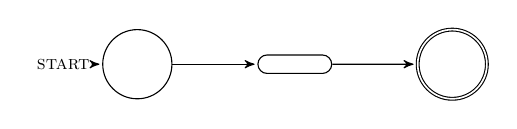
\begin{tikzpicture}[>=stealth',shorten >=1pt,auto,node distance=2cm]
					\node[initial,state]    (q0)                   {\sa};
					\node[elliptic state]   (ma)  [right of  = q0] {$\quad \ma \quad$};
					\node[state, accepting] (fa)  [right of = ma]  {\fa};
					\path[->](q0) edge (ma);
					\path[->](ma) edge (fa);
				\end{tikzpicture}
			}\\
			\subfloat[\mb]{
				\label{sfig:mb}
				\begin{tikzpicture}[>=stealth',shorten >=1pt,auto,node distance=2cm]
					\node[initial,state]    (q0)                   {\sb};
					\node[elliptic state]   (mb)  [right of  = q0] {$\quad \mb \quad$};
					\node[state, accepting] (fb)  [right of = ma]  {\fb};
					\path[->](q0) edge (mb);
					\path[->](mb) edge (fb);
				\end{tikzpicture}
			}
			\caption{
			FAs accepting $A$ and $B$.
			The middle states represent all the states of the machine other than the initial and accepting states.
			Note that if \ma or \mb accepts $\lambda$, its initial state must be an accepting state.
			}
			\label{fig:ma_and_mb}
		\end{figure}

		\noindent \textbf{(i)} \hspace{\parindent}
		We will construct an NDFA 
		\[
			M_{AB} = (Q_{AB}, \Sigma_{AB}, s_{AB}, \delta_{AB}, F_{AB})
		\]
		such that $L(\mab) = AB$.
		We build \mab by adding \mb onto the end of \ma, so that a word accepted by \mab is of the form $xy$ where $x$ is accepted by \ma and $y$ is accepted by \mb.

		Clearly, the alphabet of \mab must include all the symbols used by \ma and \mb, thus $\sigab = \siga \cup \sigb$.
		
		The states of \mab are all the states of both \ma and \mb.
		Since the names of states are meaningless, we can rename them at will. 
		Thus we can assume that \qa and \qb are disjoint, and write $\qab = \qa \cup \qb$.
		The initial state of \mab is the initial state of \ma, so $\sab = \sa$.

		The accepting states of \mab are the accepting states of \mb.
		If $\lambda$ is accepted by \mb, then \sb must be an accepting state of \mb, so that condition is accounted for
		If $\lambda$ is accepted by both \ma and \mb, we must make \sab an accepting state.
		So we define
		\[
			\fab = 	\begin{cases}
						\fb \cup \{ \sab \} &\text{if } \lambda \in A \cap B \\
						\fb &\text{otherwise}
					\end{cases}
		\]
		We have not yet accounted for the case in which $\lambda \in A$ and $\lambda \notin B$ --- doing so will require adding transitions to \mab.

		Now we must define \dalab.
		\mab should retain all the transitions of \ma and \mb, so for all $q_A \in \qa$ and $a \in \siga$, and for all $q_B \in \qb$ and $b \in \sigb$ we define
		\[
			\dalab(q_A, a) = \dala(q_A, a) \enspace \text{ and } \enspace \dalab(q_B, b) = \dalb(q_B, b).
		\]
		We also define new transitions so that any string accepted by \ma will take \mab from \sab to \sb.
		To do this, we add transitions to \sb that mimic the transitions to accepting states of \ma.
		For each transition whose result is an accepting state of \ma, we add a transition with the same origin on the same symbol leading to \sb.
		So for all $q_A \in \qa$ and $a \in \siga$ such that 
		\[
			\dala(q_A, a) \in \fa
		\]
		we define
		\[
			\dalab(q_A, a) = \sb.
		\]

		Finally, we must account for the case in which $\lambda \in A$.
		In this case, \mab must be able to skip over \ma and accept strings of $B$ without any prefix.
		Hence if $\lambda \in A$ we must create transitions from \sab which shadow the transitions from \sb.
		Thus for all $b \in \sigb$ we define
		\[
			\dalab(\sab, b) = \dalb(\sb, b).
		\]
		\begin{figure}[H]
			\centering
				\begin{tikzpicture}[>=stealth',shorten >=1pt,auto,node distance=3cm]
					\node[initial,state]    (sab)                   {\sa};
					\node[elliptic state]   (ma)  [right of = sab]  {$\quad \ma \quad$};
					\node[state]            (fa)  [right of = ma]   {\fa};

					\node[state]            (sb)  [below of = ma, node distance = 2cm]  {\sb};
					\node[elliptic state]   (mb)  [right of = sb]         {$\quad \mb \quad$};
					\node[state, accepting] (fb)  [right of = mb]         {\fb};

					\path[->](sab) edge (ma);
					\path[->](ma) edge (fa);

					\path[->](sb) edge (mb);
					\path[->](mb) edge (fb);

					\path[->](ma) edge  [out=0, in=180, below, distance=4cm]          (sb);
					\path[->](sab) edge [dashed,out=0, in=180, below, distance=2cm]   (mb);

					\node  (sab_label)   [below of = sab,node distance=1cm, text width=3cm] {\footnotesize{Accepting when\\$\lambda \in A \cap B$}};
					\node  (sab_label)   [below of = sb,node distance=1cm, text width=3cm]  {\footnotesize{Accepting when\\$\lambda \in  B$}};
				\end{tikzpicture}
			\caption{
				The dashed line is included only if $\lambda$ is accepted by \ma.
			}
			\label{fig:mab_final}
		\end{figure}
		This completes the construction of \mab.

		% AuB
		\noindent \textbf{(ii)} \hspace{\parindent}
		Now we construct an NDFA 
		\[
			M_{A \cup B} = (Q_{A \cup B}, \Sigma_{A \cup B}, s_{A \cup B}, \delta_{A \cup B}, F_{A \cup B})
		\] 
		such that $L(\maub) = A \cup B$.
		We build \maub by combining \ma and \mb in parallel, so that a string can will be accepted by \maub if it leads to an accepting state of either \ma or \mb.
		
		Clearly we need $\sigaub = \siga \cup \sigb$.

		The states of \maub are all the states of \ma and \mb, plus a new initial state \saub, which will have transitions into both \ma and \mb.
		So we define 
		\[
			\qaub = \qa \cup \qb \cup \{ \saub \}.
		\]

		We want \maub to accept strings of both $A$ and $B$, so all accepting states of \ma and \mb will be accepting states of \maub.
		If $\lambda$ is accepted by either \ma or \mb, we need \saub to be an accepting state. 
		Thus we define 
		\[
			\faub =	\begin{cases}
						\fa \cup \fb \cup \{ \saub \} &\text{if } \lambda \in A \cup B \\
						\fa \cup \fb &\text{otherwise}
					\end{cases}
		\]

		We keep all the transitions of \ma and \mb, and add new transitions linking the new initial state to the rest of the automaton.
		For each transition from the start state of \ma or \mb, we add a transition from \saub on the same symbol with the same destination.
		That is, for all $a \in \siga$ and all $b \in \sigb$, we define
		\[
			\dalaub(\saub, a) = \dala(\sa, a) \quad \text{and} \quad \dalaub(\saub, b) = \dalb(\sb, b).
		\]

		\begin{figure}[H]
			\centering
				\begin{tikzpicture}[>=stealth',shorten >=1pt,auto,node distance=3cm]
					\node[initial,state]    (sab)                             {\saub};

					\node[state]            (sa)  [above right of = sab]      {\sa};
					\node[elliptic state]   (ma)  [right of = sa]             {$\quad \ma \quad$};
					\node[state,accepting]  (fa)  [right of = ma]             {\fa};

					\node[state]            (sb)  [below right of = sab]  {\sb};
					\node[elliptic state]   (mb)  [right of = sb]         {$\quad \mb \quad$};
					\node[state, accepting] (fb)  [right of = mb]         {\fb};

					\path[->](sa) edge (ma);
					\path[->](ma) edge (fa);

					\path[->](sb) edge (mb);
					\path[->](mb) edge (fb);

					\path[->](sab) edge [out=0, in=180] (ma);
					\path[->](sab) edge [out=0, in=180] (mb);

					\node  (sab_label)   [below of = sab,node distance=1cm, text width=3cm] {\footnotesize{Accepting when\\$\lambda \in A \cup B$}};
				\end{tikzpicture}
			\caption{
				The transitions from \saub mimic those from \sa and \sb. 
			}
			\label{fig:maub_final}
		\end{figure}
		
		This completes the construction of \maub.

		% A*
		\noindent \textbf{(iii)} \hspace{\parindent}
		We construct \mas by linking \ma to itself to form a circle. % Circularize!
		Since \mas should accept strings of $A$ repeated any number of times, we allow the accepting states of \ma to behave like initial states by adding transitions from \fa looping back into \ma.
		To allow \mas to accept $\lambda$, we create a new accepting state to replace \sa as initial state.

		Let $\mas = (\qas, \siga, \sas, \dalas, \fas)$.
		Note that the alphabet of \mas is exactly the alphabet of \ma.

		We define $\qas = \qa \cup \{ \sas \}$ and $\fas = \fa \cup \{ \sas \}$, where \sas is the new initial state.

		We keep all the transitions of \ma, but for every transition from \sa, we add a transition to the same state on the same symbol from each state in \fas.
		That is, for all $a \in \siga$, and $f \in \fas$ we define 
		\[
			\dalas(f, a) = \dala(\sa, a)
		\]
		Note that since \sas is an accepting state, this also gives \sas a copy of each of the transitions from \sa.

		\begin{figure}[H]
			\centering
				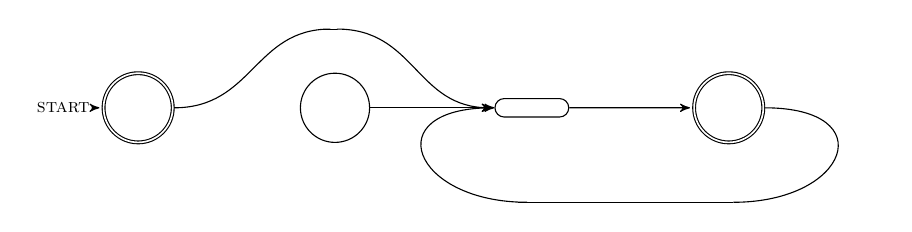
\begin{tikzpicture}[>=stealth',shorten >=1pt,auto,node distance=2.5cm]
					\node[initial,accepting,state]    (sas)                   {\sas};
					\node[state]            (sa)  [right of = sas]            {\sa};
					\node[elliptic state]   (ma)  [right of = sa]             {$\quad \ma \quad$};
					\node[state,accepting]  (fa)  [right of = ma]             {\fa};

					\path[->](sa) edge (ma);
					\path[->](ma) edge (fa);

					\node (ghost_start) [above of=sa, node distance=1cm, inner sep=0cm] {};
					\node (ghost_start2) [left of=ghost_start, node distance=0.1cm, inner sep=0cm] {};

					\path[-](sas) edge [out=0, in=180, above, distance=1cm] (ghost_start);
					\path[-](ghost_start) edge [out=0, in=180] (ghost_start2);
					\path[->](ghost_start) edge [out=0, in=180, above, distance=1cm] (ma);

					% I tried a Bezier, but I'd need more than 4 control points to get the results I want
					\node (ghost_end) [below of=fa, node distance=1.2cm, inner sep=0cm] {};
					\node (ghost_end2) [right of=ghost_end, node distance=0.2, inner sep=0cm] {};
					\node (ghost_mid) [below of=ma, node distance=1.2cm, inner sep=0cm] {};
					\node (ghost_mid2) [left of=ghost_mid, node distance=0.2cm,inner sep=0cm] {};

					\path[-](fa) edge [out=0, in=0, below, distance = 1.5cm] (ghost_end);
					\path[-](ghost_end2) edge [out=180, in=0] (ghost_end);
					\path[-](ghost_end) edge [out=180, in=0] (ghost_mid);
					\path[-](ghost_mid2) edge [out=0, in=0] (ghost_mid);
					\path[<-](ma) edge [out=180, in=180, below, distance=1.5cm] (ghost_mid);

				\end{tikzpicture}
			\caption{
				The new start state allows \mas to accept $\lambda$, while the transitions from the final states of \ma allow it to accept repeated words from $A$.
			}
			\label{fig:mas_final}
		\end{figure}

		This completes the construction of \mas.
	\end{proof}

	\begin{claim}
	\label{prop:ndfa_dfa_equivalent}
		A language is representable by an NDFA if and only if it is representable by a DFA.
	\end{claim}
	\begin{proof}
	\label{proof:ndfa_dfa_equivalent}
		Since every DFA is an NDFA, every language represented by a DFA is trivially represented by an NDFA.
		We need only prove that any language represented by an NDFA can be represented by a DFA.

		Let $M = (Q, \Sigma, s, \delta, F)$ be an NDFA.
		We will construct a DFA $M'$ such that $L(M') = L(M)$.

		Because $M$ is nondeterministic, any subset of its states may be active at any given time.
		$M'$ must have one state representing each possible set of active states of $M$, so $Q'$ must be the power set (set of all subsets, denoted $2^Q$) of $Q$.
		Thus each state in $Q'$ will be denoted by a set of the form $\{ q_1, q_2, \dots, q_n \}$ where all $q_i \in Q$.
		The initial state of $M'$ is the set $\{ s \}$, which contains only the initial state of $M$.
		The accepting states of $M'$ are the subsets of $Q$ that contain an accepting state of $M'$.

		We have defined
		\[
			M' = (Q', \Sigma, \{s\}, \delta', F')
		\]
		where
		\[
			F' = \{ p \in Q' \mid p \cap F \neq \emptyset\}.
		\]

		The only component of $M'$ remaining to be defined is $\delta'$, but it will be helpful to reexamine how we define $\delta$ before attempting to define $\delta'$.
		We defined the transition function as a mapping 
		\[
			\delta : (Q \times \Sigma) \mapsto Q.
		\]
		But this definition becomes awkward when we allow there to be any number of transitions from a given state on a single symbol.
		When dealing with NDFAs, it makes more sense to define
		\[
			\delta : (Q \times \Sigma) \mapsto 2^Q
		\]
		so that the result of each transformation is a set of states, rather than a single state.

		Given this refinement, we can define the result of each transition of $\delta'$ as a union of transitions of $\delta$.
		For each $\{ q_1, q_2, \dots, q_n \} \in Q'$ and all $a \in \Sigma$, we define
		\begin{align*}
			\delta'(\{ q_1, q_2, \dots, q_n \}, a) &= \delta(q_1, a) \cup \delta(q_2, a) \cup \dots \cup \delta(q_n, a) \} \\
			&= \bigcup_{i=1}^n \delta(q_i, a)
		\end{align*}
		
		This completes the construction of $M'$.

		Now we must prove that $L(M') = L(M)$, which is equivalent to proving that the active state of $M'$ always represents exactly the set of active states of $M$, given the same input.
		That is:
		\[
			\delta'(\{ s \}, w) = \delta(s, w) \text{ for any string } w \in \Sigma^*.
		\]
		
		We will proceed by induction on the length of the sting $w$.
		Suppose that $|w| = 0$.
		Then $w = \lambda$, and $M$ will remain in its initial state, so 
		\[
			\delta'(\{ s \}, \lambda) = \{ s \} = \delta(s, \lambda).
		\]

		Now suppose that $\delta'(\{ s \}, w) = \delta(s, w)$ for all $w \in \Sigma^*$ with $|w| \leq N$.
		Let $w \in \Sigma^*$ be of length $N$, and let $a \in \Sigma$. 
		Then $|wa| = N + 1$.
		
		We know by definition that 
		\[
			\delta'(\{ s\}, wa) = \delta'( \delta'(\{ s\}, w), a )
		\]
		and since $|w| \leq N$, we can write 
		\[
			\delta'(\{ s \}, w) = \{ p_1, p_2, \dots, p_m \} = \delta(s, w).
		\]
		Thus
		\begin{align*}
			\delta'( \delta'(\{ s \}, w), a ) &= \delta'(\{ p_1, p_2, \dots, p_m \}, a) \\
			&= \bigcup_{i=1}^m \delta(p_i, a)
		\end{align*}

		Thus we know that $\delta'(\{ s \}, w) = \delta(s, w)$ for $w$ of length $N+1$.

	\end{proof}

	\begin{claim}
	\label{prop:representable_languages_regular}
		All representable languages are regular.
	\end{claim}

	\begin{proof}
		Because we have proven that every language accepted by an NDFA is accepted by a DFA, it is enough to show that any language represented by a DFA is regular.

		Let $M = (Q, \Sigma, s, \delta, F)$ be a DFA, and let $Q = \{ q_1, \dots, q_n \}$ with $n \geq 1$.

		Define $W(i, j, k)$ to be the language containing all words that take $M$ from $q_i$ to $q_j$ without transiting any state $q_l$ with $l > k$.

		Then for $k = 0$:
		\[
			W(i, j, 0) = \{ a \in \Sigma \cup \{ \lambda \} \mid \delta(q_i, a) = q_j \}.
		\]
		That is, $W(i, j, 0)$ is the set of strings that take $M$ from $q_i$ top $q_j$ without passing through any intermediate states.
		Clearly, every element of this set must be either a symbol of $\Sigma$ or, if and only if $i = j$, the empty string.
		So for all $i$ and $j$, $W(i, j, 0)$ must be of one of the following forms:
		\begin{enumerate}[label=(\roman*), itemsep = -0.3 ex, nolistsep]
			\item $\emptyset$
			\item $\{ \lambda \}$
			\item $\{ \lambda, a_1, a_2, \dots, a_m \}, a_i \in \Sigma$
			\item $\{ a_1, a_2, \dots, a_m \}$
		\end{enumerate}
		Clearly, each of these is a regular language:
		$\emptyset$ and $\{ \lambda \}$ are atomic regular languages, and it is trivial to rewrite $\{ \lambda, a_1, a_2, \dots, a_m \}$ or $\{ a_1, a_2, \dots, a_m \}$ as the union of atomic regular languages.
		Thus $W(i, j, 0)$ is regular for all $1 \leq i, j \leq n$.

		For $k \geq 1$ we define
		\[
			W(i, j, k) = W(i, j, k-1) \cup W(i, k, k-1)\, W(k, k, k-1)^*\, W(k, j, k-1).
		\]
		That is, $W(i, j, k)$ is the union of two languages:
		The first is the language of all strings that take $M$ from $q_i$ to $q_j$ using vertices numbered less than $k$.
		The second is the language containing all stings of the form $xyz$, where $x$ takes $M$ from $q_i$ to $q_k$, $y$ takes $M$ from $q_k$ to $q_k$ and $z$ takes $M$ from $q_k$ to $q_j$, all using only states numbered less than $k$.

		Now assume that any $W(i, j, k)$ is regular for all $k \leq l$.
		We will show that all $W(i, j, l+1)$ are regular.

		For all $i$ and $j$, we know that 
		\[
			W(i, j, l+1) = W(i, j, l) \ \cup \ W(i, k, l)\ W(l+1, l+1, l)^* \ W(l+1, j, l).
		\]
		By our inductive hypothesis, we know that the languages $W(i, j, l)$, $W(i, k, l)$, $W(l+1, l+1, l)$, and $W(l+1, j, l)$ are all regular.
		Thus $W(l+1, l+1, l)^*$ is regular as the Kleene closure of a regular language, and $W(i, k, l)\, W(l+1, l+1, l)^*\, W(l+1, j, l)$ is regular as a concatenation of regular languages.
		Thus $W(i, j, l+1)$ is regular as a union of regular languages.
	\end{proof}
	

	This completes the proof of Kleene's theorem.

% chapter kleenes_theorem (end)


\mychapter{Examples Illustrating Kleene's Theorem} % (fold)
\label{sec:examples}

	\begin{example}[Mod 3 Finite Automaton]
		Constructing regular expression from the mod 3 finite automaton.
		This will help explain the proof that all representable languages are regular.

		This example will also illustrate how the numbering of the states of an FA in the inductive step of the proof of \refprop{prop:representable_languages_regular} impacts the resulting regular expression (although all possible results are equivalent, they may look very different).
	\end{example}

	\meo{
		Figure out if there are any other parts of the proof that deserve an example to help explain them.
		I will probably include pictures for regular language $\iff$ representable in the initial proof.
	}

% chapter examples (end)

\mychapter{Motivation} % (fold)
\label{sec:motivation}
	\begin{remark}
		We have seen that any regular expression is convertible into an NDFA and that any NDFA is convertible into a DFA.
		Although we have not mentioned it, there is also an algorithm to minimize any DFA: producing an equivalent automaton with a minimal number of states. 
		With a minimal DFA accepting a regular language, we can use a transition matrix to search through data for strings of that language in $\bigo(N)$ time for the amount of data, and $\bigo(m^2)$ memory for the length of the regular expression.
	\end{remark}

	\begin{remark}
		Mention the use of regular language parsing in the design of compilers and interpreters, and mention the ubiquity of \texttt{grep}.
	\end{remark}
% chapter motivation (end)



\iffalse
\mychapter{Mathematical Notation}%
\label{ch:mathematical-notation}

You may find it useful to the reader to provide a table of notation. 

\mychapter{Conclusion(s)}
\label{ch:conclusion}
\fi

% chapter conclusion (end)


%\appendix
%%% Any appendices are delineated with the \appendix command.
%%% Individual appendices are begun with the standard \chapter or
%%% \section commands.  Use an appendix for any very long argument or side issue.

\backmatter

\nocite{*}
\bibliographystyle{plainnat}
\bibliography{references.bib}

\end{document}


